\centerline{\bf \huge 8 класс}
\centerline{\bf \huge Решения}

\problem{1}
Расставьте в левой части равенства $\frac{1}{a} \quad \frac{1}{a} \quad \frac{1}{a} \quad \frac{1}{a} \quad \frac{1}{a}=(a+1)(a-1)$ знаки арифметических операций и скобки так, чтобы равенство стало верным для всех а, отличных от нуля.
%Москва 2016

\textit{Решение.}
Например, так: $\left(\frac{1}{a}:\left(\frac{1}{a} \cdot \frac{1}{a}\right)-\frac{1}{a}\right): \frac{1}{a}=(a+1)(a-1)$.

\textit{Замечание.}
Существуют и другие примеры.

\problem{2}
В примере с дробями некоторые двузначные натуральные числа заменили буквами $A$ и $B$.

$$
\frac{A-5}{A}+\frac{4}{B}=1 .
$$

(a) (1 балл) Какое наименьшее значение может принимать $A$?

(б) (2 балла) Какое наибольшее значение может принимать $B$?

\textit{Решение.} По условию

$$
1=\frac{A-5}{A}+\frac{4}{B}=1-\frac{5}{A}+\frac{4}{B}
$$


откуда получаем $\frac{A}{5}=\frac{B}{4}$ и $4 A=5 B$. Отсюда следует, что для некоторого целого $k$ имеют место равенства $A=5 k$ и $B=4 k$.

Поскольку $B=4 k \geqslant 10$, получаем $k \geqslant 3$ и $A=5 k \geqslant 5 \cdot 3=15$. Значение $A=15$ возможно, если $B=12$.

Поскольку $A=5 k \leqslant 99$, получаем $k \leqslant 19$ и $B=4 k \leqslant 4 \cdot 19=76$. Значение $B=76$ возможно, если $A=95$.

\problem{3}
Точки пересечения графиков четырех функций, заданных формулами $y=k x+b, y=k x-b, y=m x+b$ и $y= m x-b$, являются вершинами четырехугольника. Найдите координаты точки пересечения его диагоналей.
%Москва 2016

\textit{Решение.}
Графики данных линейных функций --- это две пары параллельных прямых, так как равны угловые коэффициенты у первой и второй прямой и угловые коэффициенты у третьей и четвертой прямой. Значит, точки пересечения графиков являются вершинами параллелограмма. Две противоположные вершины этого параллелограмма --- это $M(0 ; b)$ и $N(0 ;-b)$. Так как диагонали параллелограмма, пересекаясь, делятся точкой пересечения пополам, то искомая точка --- середина отрезка $M N$, то есть точка $(0 ; 0)$.

\problem{4}
В каждой клетке квадрата размером $5 \times 5$ клеток провели ровно одну диагональ. Вершина клетки свободна, если она не является концом никакой из проведённых диагоналей. Найдите наибольшее возможное количество свободных вершин.
%Москва 2019 7 класс

\textit{Решение.}

\begin{wrapfigure}{r}{0.3\linewidth}
    \vspace{-7mm}
    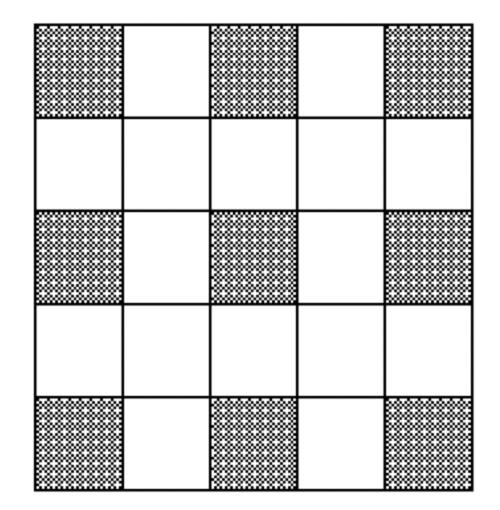
\includegraphics[width=\linewidth]{ЭлМШ 2025-2026/III блок/8/Тренировки/I/Решения/8.4.jpg}
\end{wrapfigure}

\textit{Оценка.}
Суммарное количество вершин клеток: $6 \cdot 6=36$. Выделим девять клеток, не имеющих общих вершин (см. рис. справа). Они содержат все 36 вершин. В каждой клетке проведена диагональ, поэтому в ней две вершины не свободны. Значит, использовано не менее, чем 18 вершин, поэтому свободными могут оказаться не более, чем $36-18=18$

Пример. На каждой из шести горизонтальных линий три вершины являются свободными.

\begin{center}
    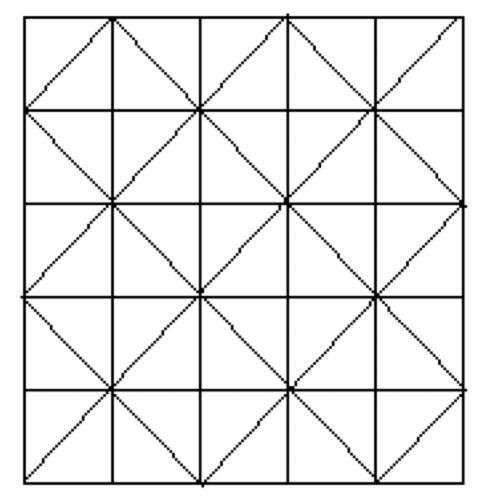
\includegraphics[width=0.4\textwidth]{ЭлМШ 2025-2026/III блок/8/Тренировки/I/Решения/8.4.1.jpg}
\end{center}


\newpage

\hspace{3mm}

\problem{5}
Дан прямоугольный равнобедренный треугольник $A B C$ с прямым углом $A$. Квадрат $K L M N$ расположен, как на рисунке: точки $K, L, N$ лежат на сторонах $A B, B C, A C$ соответственно, а точка $M$ расположена внутри треугольника $A B C$.

Найдите длину отрезка $A C$, если известно, что $A K=7, A N=3$.

\begin{center}
    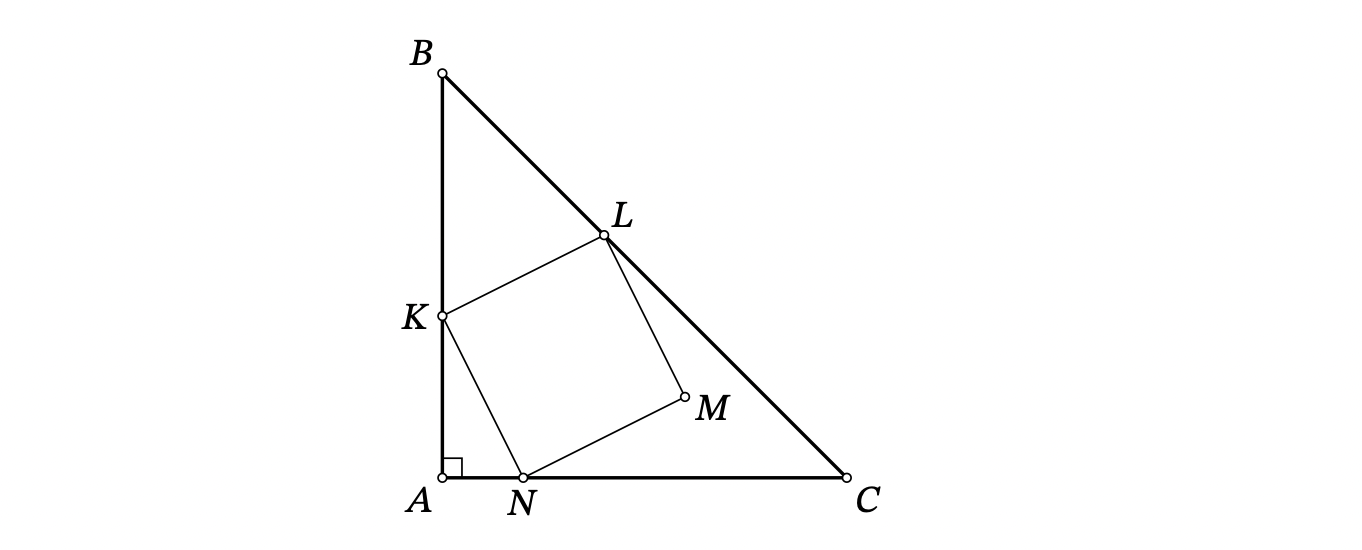
\includegraphics[width=0.7\textwidth]{ЭлМШ 2025-2026/III блок/8/Тренировки/I/Решения/8.5.png}
\end{center}
%Москва 2021

\textit{Решение.}
Решение. Отметим на отрезке $B K$ точку $H$ такую, что $L H \perp B K$ (рис. 2). Треугольник $B H L$ является прямоугольным равнобедренным, $H B=H L$. Заметим, что $\angle L K H=90^{\circ}$ - $\angle A K N=\angle A N K$, а также $K L=K N$. Прямоугольные треугольники $L K H$ и $K N A$ равны по острому углу и гипотенузе, поэтому $K H=A N=3$ и $L H=A K=7$. Следовательно,

$$
A C=A B=A K+K H+H B=7+3+7=17 .
$$

\begin{center}
    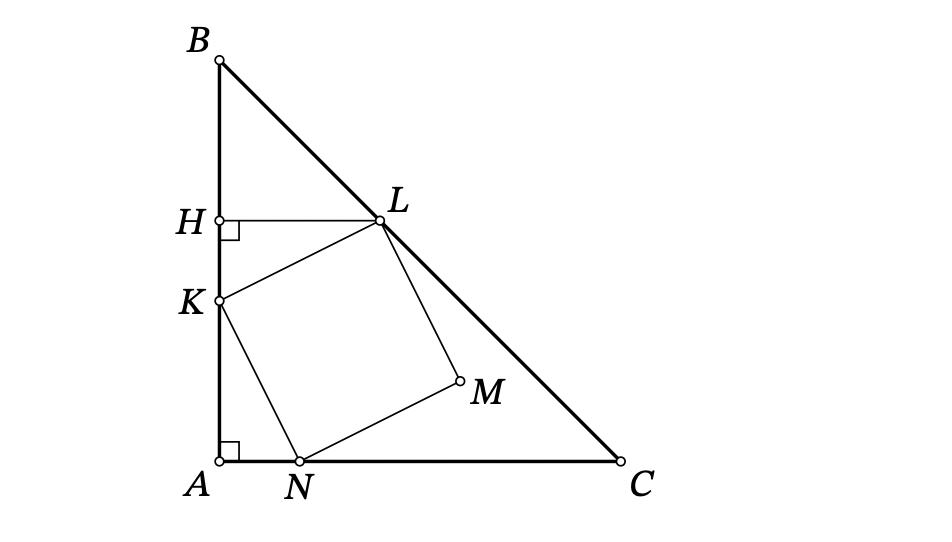
\includegraphics[width=0.7\textwidth]{ЭлМШ 2025-2026/III блок/8/Тренировки/I/Решения/8.5_sol.png}
\end{center}